\documentclass[a4paper]{article}

\def\doctitle{实验三十六\ 光源的时间相干性}

\def\docabstract{光的相干性可以分为空间上的及时间上的,时间上的相干性体现在波列的长度,这次实验会测量几种不同的光源的相干长度,加深对时间相干性的理解,并测定汞黄双线的波长差。}

\def\dockeywords{光源、相干长度、相干时间}

\usepackage{see-exp}

\def\doctoc{false}

\setlength{\parindent}{2em}

\begin{document}

%title
\input{/home/supercgor/texmf/exp-titlepage.tex}

%contents here
\begin{changemargin}{1cm}{1cm}
    \section{实验概要}
    %
    \subsection{实验目的}
    \begin{enumerate}
        \item 观测几种光源的相干长度,加深对光源时间相干性的理解
        \item 测定汞黄双线的波长差
    \end{enumerate}
    %
    \subsection{实验仪器}
    迈克尔逊干涉仪,氦氖激光器,汞灯,白炽灯,小孔光阑,扩束透镜,黄干涉滤波片,颜色玻璃。

    \subsection{实验原理}
    光源的时间相干性是由于原子发光的断续性,使得在分振幅干涉中(特别是在迈克尔逊干涉仪),两列波叠加可能并不是由同一列波分解出来,导致当光程差到达一定程度的时候,干涉的现象消失,也就是衬比度下降为零。在本次实验中,我们测量光源的相干长度$\Delta L_{max}$,然后可以测量出光源的相干时间,并利用公式:
    $$\Delta L_{max}=k(\lambda_0+\frac{\delta\lambda}{2})$$
    \section{实验数据及分析}
    \subsection{}
    \begin{spacing}{1.6}
        \begin{enumerate}
            \item 测量白光的相干长度:

                  进行本次实验前,要调整光路。首先利用“近调高低,远调俯仰”的法则,使得氦氖激光器能够水平入射干涉仪,并使激光打在干涉仪两面镜子的中央。然后调节两面镜子的方位,使得反射的激光能够原路返回激光器。如此一来,使得两面镜子是相互垂直。然后加入扩束器,转动粗调手轮,使得在屏幕上出现同心圆环的干涉条纹,一直转动粗调手轮,使得圆环被吞进原型,使得干涉条纹变粗变疏。之后微调$M_2$镜子的方位,使得其虚像$M_2^\prime$和$M_1$之间产生一个小夹角,加入白光灯以及磨砂玻璃,慢慢调出彩色的干涉条纹。

                  此时$M_1$的位置是

                  $$d_0=\SI{50.427}{\mm}$$

                  而且只看到了一级的条纹,也就是$k=1$。在这里取白光波长为

                  $$\lambda_1=\SI{550}{\nm}$$

                  再利用$\Delta L_{1max}\approx k \lambda_1$,可以得到

                  $$\Delta L_{1max} \approx \SI{5.5e-7}{\m}$$

                  相干时间$t$为

                  $$t_1=\frac{\Delta L_{1max}}{c}=\SI{1.84e-15}{\s}$$

            \item 测量白光经历橙色玻璃滤光后的相干长度

                  在上述的基础上,以经橙色玻璃滤光后的白光为入射光。在$d_0=\SI{50.427}{\mm}$的位置转动微调手轮。由光学的知识,条纹会平移,观察经过视场中心的干涉条纹,可以观察到23级的条纹。在这里取波长$\lambda_2=\SI{625}{\nm}$。可以得到
                  $$\begin{aligned}
                          \Delta L_{2max} & \approx \SI{1.44e-5}{\m} \\
                          t_3             & =\SI{4.79e-14}{\s}
                      \end{aligned}$$

            \item 测量白光经历黄干涉滤波片后的相干长度
                  和之前一样,只是用黄干涉滤波片代替橙色玻璃,可以观察到60级的条纹。在这里取波长$\lambda_3=\SI{578}{\nm}$,可以得到
                  $$\begin{aligned}
                          \Delta L_{3max} & \approx \SI{3.45e-5}{\m} \\
                          t_3             & =\SI{1.17e-13}{\s}
                      \end{aligned}$$

            \item 测量低压汞灯黄光的相干长度
                  从$d_0=\SI{50.427}{\mm}$开始,先调成等倾干涉,在视场中央出现一系列同心圆,然后转动粗调手轮。由于汞黄光是双线结构,在观测的过程中会看到一系列等间距的拍,有一个周期性的变化,但是可见度会越来越低。直到到了$d_{max}$,可见度降为零,也就是衬比度为零。在本次实验中测到的$d_{max}$为

                  $$ d_{max}=\SI{66.291}{\mm}$$

                  利用公式

                  $$\Delta L_{4max}=2(d_{max}-d_0)$$

                  可以得到

                  $$\begin{aligned}
                          \Delta L_{4max} & \approx \SI{31.728}{\mm} \\
                          t_4             & =\SI{1.058e-10}{\s}
                      \end{aligned}$$

            \item 测量汞黄双线的波长差$\Delta\lambda$
                  在等光程处附近,单方向缓慢移动粗调手轮,改变光程差,可以多次看到拍的现象以及可见度为零的点。依次记录可见度为零时,$M_1$镜子的位置读数$d_i$,数据如下表所示:

                  \begin{table}[htbp]
                      \centering
                      \captionsetup{justification=centering,margin=2cm}
                      \caption{\label{tab:tab_data2}衬比度为最低时位置实验数据表}
                      \setlength{\tabcolsep}{3mm}{
                          \begin{tabular}{cccccccc}\hline\hline
                              $i$       & 1      & 2      & 3      & 4      & 5      & 6      & 7      \\
                              $d_i$(mm) & 50.463 & 50.544 & 50.621 & 50.704 & 50.785 & 50.865 & 50.944 \\\hline\hline
                          \end{tabular}}
                  \end{table}\par

                  对上述数据做最小二乘法,可以得到以下方程:
                  $$\begin{aligned}
                          y & = 0.08x+50.38 \\
                          r & =0.9999
                      \end{aligned}$$

                  拟合的图像如下:

                  \begin{figure}[htbp]
                      \centering
                      \captionsetup{justification=centering,margin=2cm}
                      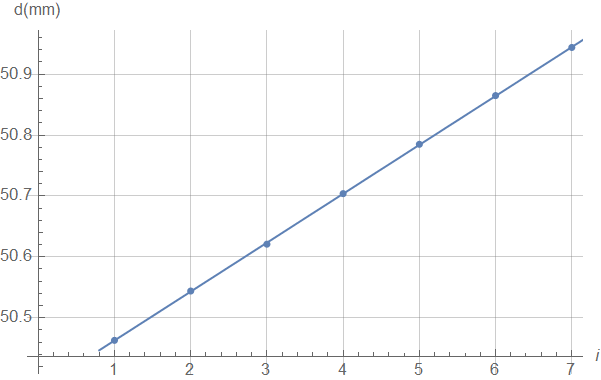
\includegraphics[width=110mm]{fig1.png}
                      \caption{\label{fig:1}衬比度最低时位置拟合图}
                  \end{figure}

                  由此可以得到
                  $$\Delta d=\SI{0.08}{\mm}$$
                  在这里取波长$\lambda_5=\SI{578.01}{\nm}$,利用公式
                  $$\Delta\lambda=\frac{\lambda^2}{\Delta d}$$
                  可以得到
                  $$\Delta\lambda=\SI{2.09}{\nm}$$

            \item 	利用光电自动记录画出的干涉图,测量$\Delta\lambda$

                  干涉图由实验室提供,可以数出干涉条纹数目$\Delta k=270$。利用公式
                  $$\Delta\lambda=\frac{\lambda}{\Delta k}$$
                  可以得到
                  $$\Delta\lambda=\SI{2.14}{\nm}$$

                  由此可见,两种方法测量的$\Delta\lambda$十分接近。
        \end{enumerate}
    \end{spacing}

    \subsection{思考题}
    \begin{spacing}{1.6}
        \begin{enumerate}
            \item 用汞黄双线的光照明干涉仪,为什么可见度随光程差做周期变化?而且逐渐衰减到零?

                  讨论这个问题可以简化模型,假设照射的光是两个频率不一样的单色光进行非相干叠加。可以得到叠加之后的衬比度为
                  $$\gamma=|\frac{\sin(\pi\frac{\mathrm{\Delta L}}{L_0})}{\pi\frac{\mathrm{\Delta L}}{L_0}}|$$
                  其中$L_0$是相干长度,$\mathrm{\Delta L}$是光程差。从上面的公式可以解释可见度,其实就是衬比度为什么会做周期性变化,以及随着光程差增大而衰减到零。

            \item 本次实验的误差来源

                  判断条纹是不是消失是具有很大的主观性,而且每一次观测的结果都不一定一样。
                  实验使用的迈克尔逊干涉仪有比较大的空程差,逆时针和顺时针扭动粗调手轮所测得的数据有比较大的区别。
                  干涉条纹的观测有机会不在视场中心,在数条纹个数时容易有误差。
        \end{enumerate}
    \end{spacing}
    \subsection{感想}
    \begin{spacing}{1.6}
        \hspace{2em}本次实验是上学期迈克尔逊干涉仪实验的后续,经过本次实验进一步加深了对于迈克尔逊干涉仪的认识,同时对时间相干性这一个深刻的物理概念有了更加深入地体会。感谢老师在本次实验的指导,并且检查了实验中的数据。
    \end{spacing}










\end{changemargin}
\end{document}